\chapter{ART Internals: App Executable Format}
\label{chapter:art_oat_file_inspection}

A core element of the recently introduced ART is the file that
gets created by ``dex2oat'' during the installation time of an app,
described in \autoref{section:app_installation}.
Since ART does use AOT compilation, the file format is expected
to be an executable or at least a native code container.
A lot of copy protection mechanisms are based on the use of native
code because it is supposed to be more secure from reverse code
engineering (which is an assumption so far).
Therefore it's worth to have closer look at that file format
especially since Google does not provide any further information
about it's content and it might have the potential of
revolutionizing the available copy protection mechanisms for
Android or having at least a great impact on them.

By applying the Unix command ``\code{file}'' (which can classify
files to MIME-types) to the resulting file of the ``\code{dex2oat}''
tool it comes apparent that it's a particular ELF file (32 or 64 bit)
called OAT file from now on.

\section{ELF File Format}\label{section:elf_file_format}
ELF originally was originally specified by UNIX System Laboratories
(USL) and later by Tool Interface Standards (TIS) and is a common
standard for executables, object code and shared libraries on UNIX
systems. It's a quite flexible format for different CPUs and
architectures and does serve as a container for different
executable binary formats.

\begin{figure}[htb]
  \centering
  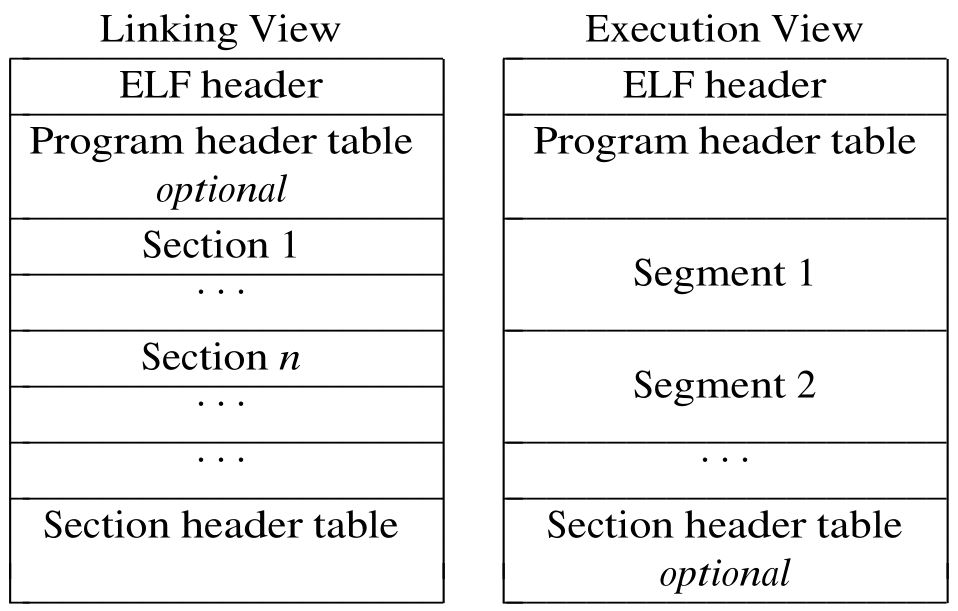
\includegraphics[scale=0.4]{figures/elf_format}
  \caption[ELF file format]{ELF file format taken from \parencite{portable_formats_spec}}
  \label{fig:elf_format}
\end{figure}

The \autoref{fig:elf_format} shows the file structure.
One have to differentiate the context of how the file is viewed.
While a linker does care about sections, sections may be
glued together to segments when executing the file.
Meta data about the file can be read out of the ``ELF header''
that starts at adress \code{0x00} and does contain
information about the version, file type, target machine and
offsets to the program- and section header tables.
In ART, the file is marked as an shared object with LSB encoding
and not as an executable which makes clear that this file is not
supposed to get executed directly but to be linked first
(An open question remains so far which process is then starting
the app).
Segments are referenced by the program header table and sections
by the section header table. For an execution process, only the header
and the information out of the program header table is needed
\parencite{life_of_binaries}.

Let's first have a look at the used sections in case of the specific
Android implementation, the OAT file:
\autoref{fig:section_headers} does show the output of
``\code{readelf -S <ELF-App-File>}'', listening all available sections

\begin{figure}[htb]
  \centering
  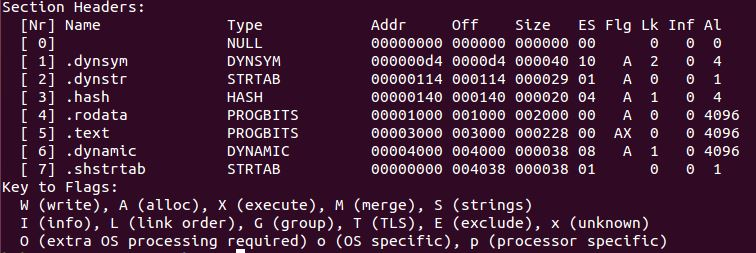
\includegraphics[width=\textwidth]{figures/android_elf_section_headers}
  \caption[ELF section headers]{ELF section headers}
  \label{fig:section_headers}
\end{figure}

It does follow a short description of sections that are implemented
\parencite{life_of_binaries}:
\begin{itemize}
    \item \code{.dynsym} holds a dynamic linking symbol table that
    does contain information for locating and relocating a program's
    symbol definitions and references. It does contain ``oatdata'',
    ``oatexec'' and ``oatlastword'' in case of an OAT file.
    \item \code{.dynstr} does hold strings for dynamic linking,
    mostly names that are referenced by \code{.dynsym}.
    \item \code{.hash} contains the symbol hash table
    \item \code{.rodata} stands for ``Read-Only data'' and does
    contain arbitrary data whose interpretation is solely
    determined by the program itself. We will
    see that in case of Android it does hold the actual OAT file
    that will be further described in \autoref{section:oat_file}.
    \item \code{.text} is the only region that is marked as
    executable and therefore it does hold the main body of
    program code.
    \item \code{.dynamic} includes dynamic linking information.
    \item \code{.shstrtab} stands for ``Section header string
    table'' and therefore contains the previous described
    section names including its own (e.g. ``\code{.shstrtab}'').
\end{itemize}

\autoref{fig:program_headers} shows the alternative view of the
file by having a look at segments (``\code{readelf -S <ELF-App-File>}'')
. Type ``PHDR'' stands for ``Program header''. Segments with type
``LOAD'' are supposed to be loaded from disk into memory while
a ``DYNAMIC'' segment is a part of a ``LOAD'' segment and is equal
to the ``\code{.dynamic}'' section. The mapping of ``LOAD'' segments
into memory is performed by respecting the alignment of \code{0x1000}
means that only chunks of that size (or a multiple) are being read
(e.g. reading the segment at \code{0x3000} will copy the content
from \code{0x3000-0x4000} even if the size only equals \code{0x340}).
The difference between ``FileSiz'' that obviously stands for the file
size and ``MemSiz'' that stands for memory size is the space that
gets reserved for uninitialized variables.
\begin{figure}[htb]
  \centering
  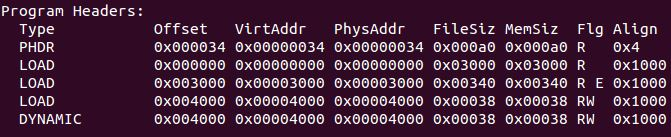
\includegraphics[width=\textwidth]{figures/android_elf_program_headers}
  \caption[ELF program headers]{ELF program headers}
  \label{fig:program_headers}
\end{figure}
The \code{readelf} tool is also capable of showing the resulting
mapping of sections to segments
(\autoref{fig:sections_segments_mapping}).

\begin{figure}[htb]
  \centering
  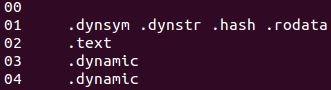
\includegraphics[scale=0.7]{figures/section_segment_mapping}
  \caption[ELF section segment mapping]{ELF section segment mapping}
  \label{fig:sections_segments_mapping}
\end{figure}

It's interesting to note that the Android usage of ELF for apps
is very minimalistic and does contain very few sections/segments
compared to a common program written in C/C++ (\code{helloWorld.c}
does include over 30 sections). As described before,
\code{.dynsym} does contain entries which tell us where to find
the OAT data, specifically the ``oatdata''(equals \code{.rodata})
and the ``oatexec'' (equals \code{.text})
section that will now be analyzed.

\section{OAT File}\label{section:oat_file}
Google does not provide any official documentation about the OAT
file format other than the source code itself
(\code{art/runtime/oat[\_file].h[c]}). \parencite{hiding_behind_art}
however gives a helpful introduction and an overview is given
in \autoref{fig:oat_format} that shows the content of ``oatdata''.

\begin{figure}[htb]
  \centering
  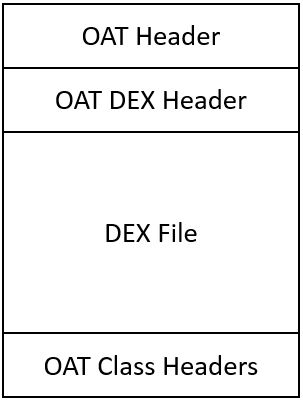
\includegraphics[scale=0.5]{figures/oat_format}
  \caption[OAT format]{OAT format}
  \label{fig:oat_format}
\end{figure}

Important attributes that the ``OAT Header'' contains are the
checksum over itself,
the instruction set (ARM, ARM64, MIPS, \ldots), the executable
offset from start of ``oatdata'' and the quantity of embedded
DEX files (that should be one and does exist for flexibility
reasons). It does follow the ``OAT Dex Header'', containing
the absolute path of the original DEX file, the checksum, the
offset to the copy of the DEX file that is embedded as well as
an offset to the ``OAT Class Headers''. ``OAT Class Headers''
do offer information about defined classes. First, the type
of class which contains how many methods in the class
are compiled to native code (``all'', ``some'' or ``none'' but
should be ``all'' in almost every case) and secondly
the offsets to the native code begin of every compiled method.
The actual code is located in a superordinated section
(\code{.text}) which is seperated but referenced from this one.

\section{DEX File Format}
\label{section:dex_file_format}
To be complete, we will also have a quick look into the DEX format,
which is officially documented by Google \parencite{dex}.
Before the introduction of ART, DEX was the last unit before
execution of an app (besides ODEX). However, the DVM does accept
both formats thats why it is possible to dynamically execute
DEX without the transformation step. DEX does not only contain
the VM instructions but some meta data to locate
higher abstaction level information like classes and within that
methods, fields, \ldots.

\autoref{fig:dex_format} does show the file layout.
\begin{figure}[htb]
  \centering
  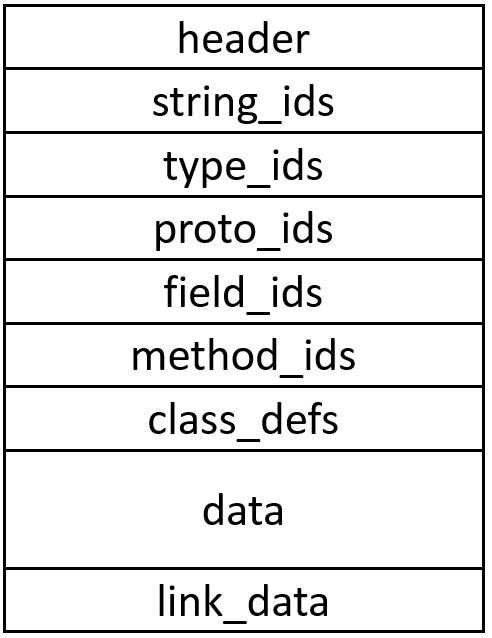
\includegraphics[scale=0.3]{figures/dex_format}
  \caption[DEX format]{DEX format}
  \label{fig:dex_format}
\end{figure}
The header again includes a checksum of the whole file (checksum
field excluded), the overall size as well as the offsets and sizes
of every section. Sections with ``ids'' ending are arrays of
id items of their type and do reference
a data item in the ``data'' section or are specifying
an index into another ``ids'' section. A ``string\_id'' item for
instance does just contain an offset from file beginning
that should be located in ``data'' whereas the ``type\_id'' item
includes an index into the ``string\_ids'' field. The principle
of the file structure is therefore a nesting architecture of
sections. The ``class\_def'' section does contain methods that
in turn include strings, fields and so on. Content is being
stored exclusively in the data section. In the end,
executable VM instructions are referenced from methods.


\section{Conclusion}\label{section:andelf_format_conclusion}
The runtime transition from DVM to ART of course had to result
in a new file that gets intepreted/executed when an app starts.
However, the change is not as smooth as expected since
the new file format is not pure executable code but, as
discovered in this chapter, a combination of native code
and embedded DEX code as well as a new OAT file format
which references parts of the native code. Also, there is some
confusion for what part the name ``OAT file'' stands. On the
one hand, Google's documentation files and the naming
convention of the``dex2oat'' tool are giving the impression
that the file as a whole is an ``OAT file''. On
the other hand, the file is a valid implementation of the
well known ELF format and contains a section that starts
with bytes known by MIME types with ``.oat'' as file format
(.rodata section). Additional, the ``oatexec'' section
is controlled via the greater ELF format. Therefore
, ``OAT file'' stands most likely for both of those meanings, the
Android app specific and minimalistic implementation of the ELF
as well as the combination of the ``oatdata'' and ``oatexec''
section to a file alike entity. \autoref{fig:andelf_format} does
provide an overall view of the fileformat of ART app executables.

\begin{figure}[htb]
  \centering
  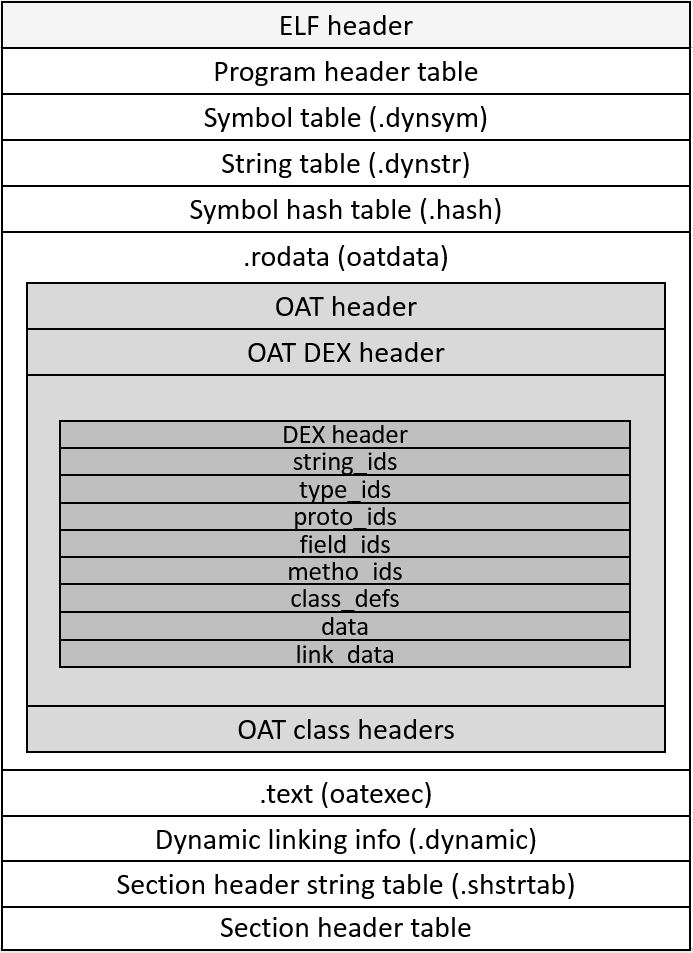
\includegraphics[scale=0.5]{figures/andelf_format}
  \caption[ART app executable format]{ART app executable format}
  \label{fig:andelf_format}
\end{figure}

The awareness of the detailed executable file format does pop
new questions about the ART Android internals.
Since the file is marked as an shared object, it won't get
executed as a standalone program but most likely will be also
included in a forked Zygote process like in the Dalvik runtime.
However it is not clear which parts of the OAT file are
needed to run an app adequately. Is the embedded DEX for instance
mandatory for the app to work correctly? As we have seen in
\autoref{chapter:copy_protection_status_quo}, DEX files are
a crucial part of applications to protect. What if that part
can be missed out by distributing a minimal stub application
followed by a dynamic native code injection at runtime?
It is also interesting if and how the known dynamic obfuscation
techniques, described in \autoref{section:obfuscation_techniques},
can be applied to ART apps since there is no VM bytecode that can
be manipulated at runtime but only native code.
Therefore a deep understanding for the app init and execution
process under ART is a precondition to answer these
questions and has to be way more detailed than described in
\autoref{section:app_execution}.
